\chapter{Uvod}
\label{ch:uvod}

\section{Problem i motivacija}

Renderovanje u realnom vremenu dominantno se zasniva na rasterizaciji, koja veoma efikasno
razre\v{s}ava primarnu vidljivost (\v{s}ta kamera neposredno vidi), ali nema nikakav prirodan pojam o tome
\v{s}ta bilo koja ta\v{c}ka povr\v{s}i vidi izvan sebe. Efekti po kojima slika deluje verodostojno zavise upravo
od toga: indirektno osvetljenje koje se odbija izme\dj u povr\v{s}i, kontaktne senke, sjajne refleksije i
ambijentalna okluzija svi odgovaraju na pitanje \quotedblbase{}\v{s}ta je jo\v{s} vidljivo odavde\textquotedblright{}. Engine-i za
renderovanje u realnom vremenu odavno ih aproksimiraju. Metode u prostoru ekrana (SSAO, refleksije i
globalno osvetljenje u prostoru ekrana) su jeftine, ali vide samo ono \v{s}to je trenutno na ekranu, pa
otkazuju kad je potrebna geometrija van ekrana ili tek otkrivena disokluzijom
\cite{mittring2007cryengine, bavoil2008hbao}. Prora\v{c}unate metode pe\v{c}u osvetljenje u lightmape ili
probe i ne mogu da prate dinami\v{c}ku geometriju. Voksel pristupi, kao \v{s}to je voxel cone tracing, pokrivaju
celu scenu, ali su grubi i skloni curenju svetlosti \cite{crassin2011vxgi}.

Hardversko pra\'cenje zrakova menja ono \v{s}to je isplativo. GPU-ovi od NVIDIA RTX (2018) i AMD RDNA2 (2020)
imaju namenske jedinice za obilazak hijerarhije grani\v{c}nih zapremina (BVH) i presek zraka i trougla, pa je
zrak prema celoj sceni dovoljno jeftin da se baca po pikselu interaktivnom brzinom. Navedeni efekti
postaju fizi\v{c}ki zasnovani prolazi koji uzorkuju stvarnu scenu umesto proksija u prostoru ekrana.
Problem je cena. Direktno re\v{s}avanje jedna\v{c}ine renderovanja \cite{kajiya1986rendering} path tracing-om,
koji integrali svetlost koja sti\v{z}e u ta\v{c}ku povr\v{s}i iz svih pravaca, ostaje daleko izvan bud\v{z}eta
realnog vremena pri rezoluciji ekrana. Prihvatljiv bud\v{z}et je jedan ili nekoliko zrakova po pikselu, \v{s}to
uzorkuje samo mali deo putanja svetlosti koje sti\v{z}u u piksel, pa je procena ta\v{c}na u proseku, ali ne i po
pikselu. Ta gre\v{s}ka je \v{s}um. Prakti\v{c}an put, kojim ide i ovaj rad, zato je hibridan: primarna
vidljivost se rasterizuje, sekundarni efekti se dodaju kao prolazi sa pra\'cenjem zrakova pri malom broju
uzoraka, a \v{c}ista slika se rekonstrui\v{s}e uklanjanjem \v{s}uma \cite{schied2017svgf}
(Slika~\ref{fig:teaser}).

\begin{figure}[tbp]
\centering
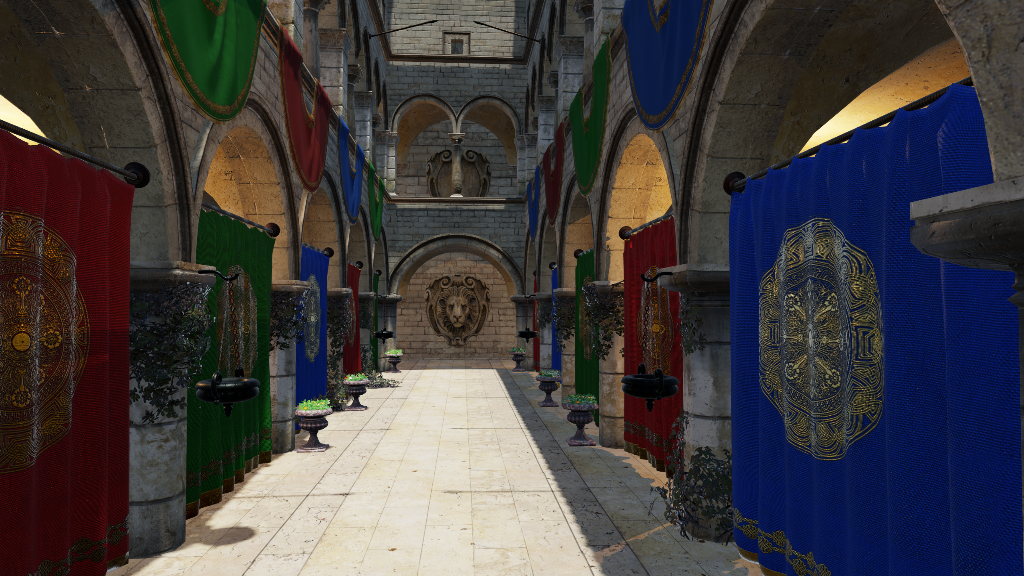
\includegraphics[width=0.92\textwidth]{figures/teaser_raster.png}\\[2mm]
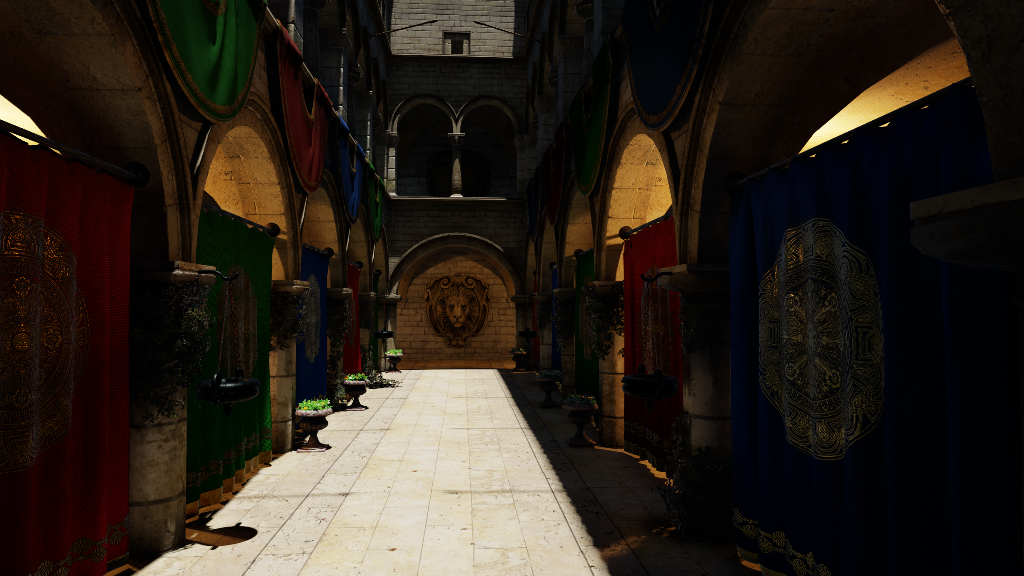
\includegraphics[width=0.92\textwidth]{figures/teaser.png}
\caption[Isti kadar rasterizovan i sa osvetljenjem zasnovanim na pra\'cenju zrakova]{Isti kadar, kamera i
ekspozicija na test sceni (Sponza). \textbf{Gore:} sam rasterizovani forward prolaz, u kome konstantan
ambijentalni \v{c}lan zamenjuje sve \v{s}to svetlost radi posle prvog odbijanja. \textbf{Dole:} isti prolaz sa
senkama, ambijentalnom okluzijom, refleksijama i globalnim osvetljenjem zasnovanim na pra\'cenju zrakova.
Gornja slika je svetlija, \v{s}to je i poenta: njen ambijentalni \v{c}lan podjednako podi\v{z}e svaku povr\v{s}inu,
osvetljenu ili ne, dok ga na donjoj zamenjuje svetlost koja je stvarno pre\v{s}la put.}
\label{fig:teaser}
\end{figure}

\section{Za\v{s}to hibridni pristup i za\v{s}to ray query (a ne RT pipeline)}

Vulkan nudi dva na\v{c}ina za pra\'cenje zrakova: namenski ray tracing pipeline i inline ray query
(\texttt{VK_KHR_ray_query}). Odeljak~\ref{sec:vulkanrt} ih poredi.

Ovaj rad koristi inline ray query iz razloga arhitektonske uklopljenosti: engine je rasterizacioni forward
renderer, a inline upiti omogu\'cavaju da se svaki efekat ubaci kao obi\v{c}an compute ili fragment prolaz,
bez preure\dj{}ivanja renderera oko ray tracing pipeline-a i njegove tabele vezivanja. Efekti se mogu
dodavati jedan po jedan, \v{s}to odgovara hibridnom dizajnu u kome su zraci ciljani dodatak rasterizaciji, a
ne primarna arhitektura. Cena je to \v{s}to se rad sa zracima ne mo\v{z}e preure\dj{}ivati izme\dj u invokacija
\v{s}ejdera radi o\v{c}uvanja koherentnosti divergentnih putanja, i to \v{s}to rekurzija mora biti eksplicitna
petlja, a ne \v{s}ejder koji pokre\'ce novi zrak. Efekti ovde su plitki (jedno odbijanje), pa je druga cena
mala.

\section{Cilj i istra\v{z}iva\v{c}ko pitanje}

Cilj je da se implementiraju \v{c}etiri efekta osvetljenja zasnovana na pra\'cenju zrakova: senke,
ambijentalna okluzija, refleksije i difuzno globalno osvetljenje, kroz inline ray query u sopstvenom Vulkan
engine-u, i da se svaki od njih okarakteri\v{s}e. Istra\v{z}iva\v{c}ko pitanje se razla\v{z}e na merljiva potpitanja:
cena svakog efekta na GPU-u u milisekundama; uticaj broja uzoraka po pikselu na kvalitet (PSNR/SSIM) i na
vreme; kvalitet i cena uklanjanja \v{s}uma kad je uklju\v{c}eno u odnosu na isklju\v{c}eno; uticaj pra\'cenja zrakova pri
polovini u odnosu na punu rezoluciju; i kako se identi\v{c}na Vulkan implementacija pona\v{s}a na GPU-ovima
razli\v{c}itih proizvo\dj{}a\v{c}a (AMD RDNA4 prema NVIDIA Blackwell). Obim je namerno ograni\v{c}en: jedna
zatvorena scena (Sponza), dva GPU-a aktuelne generacije sli\v{c}nog ranga (Tabela~\ref{tab:gpus}), difuzno
globalno osvetljenje i konvergirana path-traced referenca za metrike kvaliteta.

Tri odgovora protivre\v{c}e intuiciji. Osam puta ve\'ci bud\v{z}et zrakova donosi samo \rcPsnrGain{} dB PSNR-a.
Dobitak je stvaran, jer pribli\v{z}no tri puta prema\v{s}uje prag merenja, ali ko\v{s}ta \rcGpuPct\% vi\v{s}e GPU
vremena, pa radnu ta\v{c}ku postavlja na jedan zrak po pikselu (Odeljak~\ref{sec:raycount}). Uklanjanje
\v{s}uma se isplati u temporalnoj stabilnosti, a ne u stati\v{c}koj vernosti (Odeljak~\ref{sec:motion}). I
\v{s}ejder koji nosi inline upit za senke zauzima 130 registara prema 87 bez njega, \v{s}to prelazi granicu
alokacije i spu\v{s}ta ga sa 16 istovremeno rezidentnih talasa na 10, a upravo tu se cena tog upita
stati\v{c}ki vidi (Odeljak~\ref{sec:occupancy}).

\section{Doprinosi}

Doprinosi su:

\begin{itemize}
\item integrisana implementacija \v{c}etiri hibridna efekta osvetljenja zasnovana na ray query-ju, otvorene
licence, u jednom sopstvenom Vulkan engine-u;
\item raspodela cene GPU-a po efektima dobijena ponovljivim A/B benchmark okvirom, a ne ad hoc
snimcima;
\item ponovo upotrebljiv obrazac sa polovinom rezolucije, prepass-om G-bafera, uklanjanjem \v{s}uma i
upsampling-om;
\item evaluacija sopstvene implementacije SVGF filtera koji dele svi signali kojima je potreban: kvalitet
koji vra\'ca, cena i temporalna stabilnost;
\item pore\dj{}enje performansi istog koda identi\v{c}nog ray query pipeline-a na AMD RDNA4 i NVIDIA Blackwell
hardveru, koje pokazuje da se rang dve strategije senki me\dj{}u proizvo\dj{}a\v{c}ima obr\'ce
(Odeljak~\ref{sec:analiza-shadow-strategy}, Tabela~\ref{tab:shadow-strategy}): stohasti\v{c}ka strategija
pobe\dj{}uje za \perfShadowGapAMD{} ms na RX 9070 XT, a gubi za faktor \perfShadowRatioNV{} na RTX 5070.
\end{itemize}

\section{Struktura rada}

Glava~\ref{ch:pregled} daje pregled teorijskih osnova (rasterizacija prema pra\'cenju zrakova, strukture
ubrzanja, Vulkan ekstenzije za pra\'cenje zrakova) i postoje\'ca re\v{s}enja u realnom vremenu sa kojima se
evaluacija poredi. Glava~\ref{ch:implementacija} opisuje implementaciju: engine i graf renderovanja,
izgradnju struktura ubrzanja, \v{c}etiri efekta, SVGF filter, temporalni resolve i alate za merenje.
Glava~\ref{ch:analiza} izoluje cenu svakog efekta i meri kvalitet rekonstrukcije u odnosu na referencu i na
postoje\'ca re\v{s}enja iz Glave~\ref{ch:pregled}. Glava~\ref{ch:zakljucak} iznosi ograni\v{c}enja i
pravce daljeg rada.
